\section{Spice Impedance Synthesis}\label{spice_impedance_synthesis}

This project brings toghether a sequence of processes so that tabulated frequency domain complex impedance data can be used to determine a Spice sub-circuit which reproduces the impedance function. The process requires the following software to be installed in order to run correctly:

\begin{enumerate}

\item VECTOR\_FIT software (https://github.com/chrissmartt/vector\_fit)

\item NETWORK\_SYNTHESIS softwatre (https://github.com/chrissmartt/network\_synthesis)

\item Ngspice software (http://ngspice.sourceforge.net/)

\item gnuplot software (http://www.gnuplot.info/)

\end{enumerate}

The spice\_impedance\_synthesis process is found in the TEST\_DATA directory

The script spice\_impedance\_synthesis runs the vector fit process with a given model order
and then the network synthesis process to produce a Spice circuit model. The Spice circuit model
is run using ngspice to determine the complex impedance produced by the Spice model.

The comparison between the input data and the vector fit
model data is plotted, then the comparison between the Spice model data 

The complex frequency domain data should be in an ascii file with three columns: frequency, real part of the function at this frequency, imaginary part of function at this frequency. Data for each frequency should be on a sperate line. An example file is shown below:

\begin{verbatim}
   1000.00000       8.50000009E-02  -159.154678         
   1059.56042       8.50000009E-02  -150.208176         
   1122.66772       8.50000009E-02  -141.764648         
   1189.53442       8.50000009E-02  -133.795685         
   1260.38281       8.50000009E-02  -126.274742         
       .                .                 .
       .                .                 .
       .                .                 .
   79340968.0       8.50000009E-02   21.4340954         
   84066512.0       8.50000009E-02   22.7109394         
   89073600.0       8.50000009E-02   24.0638466         
   94378816.0       8.50000009E-02   25.4972954         
   100000000.       8.50000009E-02   27.0161057         
\end{verbatim}

The output of the process is a Spice subcircuit file (impedance.lib) An example is shown below:

\begin{verbatim}
* Spice sub-circuit model for impedance created by NETWORK_SYNTHESIS software
* https://github.com/chrissmartt/network_synthesis
* 
.subckt impedance_model 1 10000
C01      1     2  4.6566E-09
R01      1     2  1.1869E+00
*
C02      2     3  1.0406E-05
R02      2     3  1.0000E+08
*
L03      3     4  2.5654E-09
*
R04      4     5  5.1045E-01
*
L05      5 10000  3.5720E-08
*
R06      5 10000  2.0690E+03
*
C07      5     6  4.7762E-12
R07      5     6  1.0000E+08
*
R08      6     7  5.2972E+00
*
R09      7     8  1.1457E+00
C09      8 10000  4.7061E-12
*
L10      7 10000  2.1245E-09
*
R11      7 10000  6.5808E+02
*
*
.ends
\end{verbatim}

\subsection{Example}

The file CAPACITOR\_Z\_measured\_plus\_LF\_model.CSV contains complex impedance data for
a capacitor from 10Hz to 3GHz. This is a combination of measured data from a VNA (300kHz to 3GHz) plus an extrapolation to low frequency assuming the impedance takes the form $Z=R+\frac{1}{(j \omega C)}$.

\vspace{5mm}

Run the test case with:

\vspace{5mm}

spice\_impedance\_synthesis CAPACITOR\_Z\_measured\_plus\_LF\_model.CSV 6

\vspace{5mm}

The following plots show the comparison between the input impedance data and the vector\_fit approximation then the input impedance data and the results of the Ngspice simulation using the derived Spice sub-circuit model.

\begin{figure}[h]
\centering
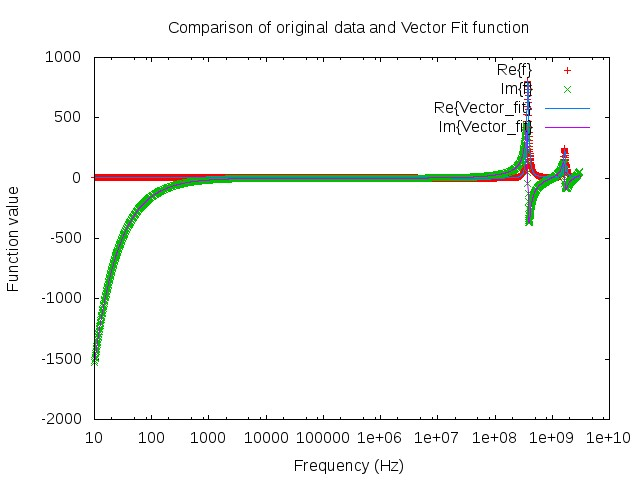
\includegraphics[scale=0.75]{./Imgs/Z_Vfit.jpg}
\caption{Comparison of input impedance data with the 6th order pole-residue approximation produced by the vector fitting process}
\label{fig:Z_Vfit}
\end{figure}

\begin{figure}[h]
\centering
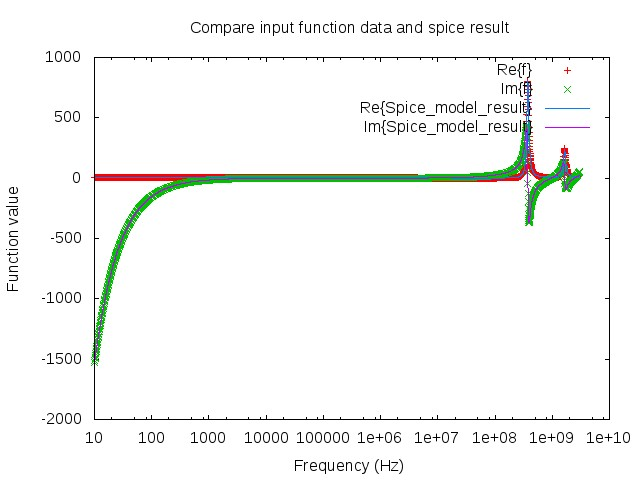
\includegraphics[scale=0.75]{./Imgs/Z_spice.jpg}
\caption{Comparison of input impedance data with the Ngspice simulation of the Spice subcircuit impedance model}
\label{fig:Z_Vfit}
\end{figure}

 
